\chapter{El grupo fundamental}%
\label{cha:el_grupo_fundamental}
\section{Operaciones con caminos}%
\label{sec:operaciones_con_caminos}
Sea $X$ es conexo por caminos.
\begin{defi}[Producto]
$\sigma, \tau: \left[ 0, 1 \right] \rightarrow X, \sigma\left( 1 \right) = \tau\left( 0 \right) \Rightarrow \sigma * \tau\left( t \right) = \begin{cases}
    \sigma\left( 2 t \right),\ 0 \le t \le 1/2\\
    \tau\left( 2t - 1 \right),\ 1/2 \le t \le 1
\end{cases}$

[Reescalando $\begin{cases}
    \sigma \text{ de } \left[ 0, 1 \right] \text{ a } \left[ 0, 1/2 \right]\\
    \tau \text{ de } \left[ 0, 1 \right] \text{ a } \left[ 1/2, 1 \right] 
\end{cases}$]

%TODO: Imagen
\begin{center}
    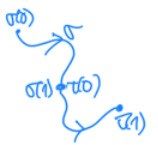
\includegraphics[scale=0.3]{images/prod_grupo_fundamental} 
\end{center}
\end{defi}

Las propiedades algebraicas son TODAS SALVO HOMOTOPÍA \underline{CON EXTREMOS FIJOS}.
%TODO: Fix
\begin{prop}
\underline{Propiedades} de grupo:
\begin{enumerate}
    \item \underline{Asociativa}: $\left( \alpha * \beta \right) * \gamma \simeq \alpha * \left( \beta * \gamma \right)$.

    En cada altura $s$ se reescalan los caminos con junturas.
    \begin{center}
        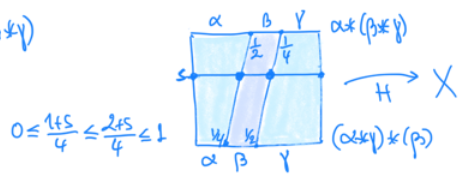
\includegraphics[scale=0.3]{images/asoc_gr_fund} 
    \end{center}
    \item \underline{Neutros}: 
    \begin{center}
        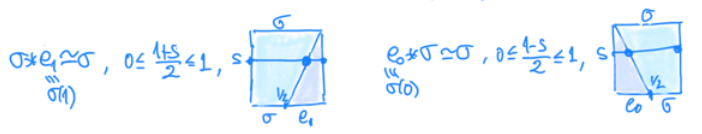
\includegraphics[scale=0.3]{images/neutro_gr_fund} 
    \end{center}
    \item \underline{Inverso}: $\sigma'\left( t \right) = \sigma\left( 1 - t \right) \Rightarrow \sigma * \sigma' \simeq e_0$ y $\sigma'' = \sigma \Rightarrow \sigma' * \sigma \simeq e_1$.

    No se reescala: $0 \le \frac{1 - s}{2} \le \frac{1 + s}{2} \le 1$. 

    Las junturas dicen dónde parar $\sigma$ y empezar $\sigma'$ en cada altura:
    \begin{center}
        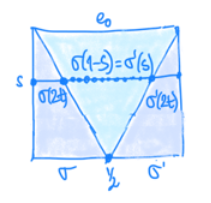
\includegraphics[scale=0.3]{images/inv_gr_fund} 
    \end{center}

    \item \underline{Invarianza por homotopía}: 
    \begin{gather*}
        \begin{cases}
            F_s: \sigma_1 \simeq \sigma_2\\
            G_s: \tau_1 \simeq \tau_2
        \end{cases} \xRightarrow{\text{Trans.}} F_s * G_s: \sigma_1 * \tau_1 \simeq \sigma_2 * \tau_2\\
        F_s * G_s\left( t \right) = \begin{cases}
            F_s\left( 2t \right),\ 0 \le t \le \frac{1}{2},\\
            G_s\left( 2t - 1 \right),\ \frac{1}{2} \le t \le 1
        \end{cases} 
    .\end{gather*}

\end{enumerate}
\end{prop}

\section{El grupo fundamental}%
\label{sec:el_grupo_fundamental}
Sea $X$ conexo por caminos, $x_0 \in X$ \underline{punto base} fijo.
\begin{defi}
\begin{enumerate}
    \item \underline{Lazo de base $x_0$}, $\sigma: \left[ 0, 1 \right] \rightarrow X,\ \underbrace{\sigma\left( 0 \right) = \sigma\left( 1 \right)}_{\text{lazo}} = x_0$, punto fijo.

    \item \begin{itemize}
        \item $\sigma, \tau: \left[ 0, 1 \right] \rightarrow X$ lazos de base $x_0$.
        \item $H_s: \sigma \simeq \tau$ \underline{de lazos}: $H_s\left( 0 \right) = H_s\left( 1 \right),\ \forall s$.
        \item $H_s = \sigma \stackrel{x_0}{\simeq} \tau$ de lazos \underline{con punto base fijo}: $H_s\left( 0 \right) = H_s\left( 1 \right) = x_0,\ \forall s$. [Relativa a $\{0, 1\}$]
    \end{itemize}
\end{enumerate}
\end{defi}
\begin{defi}[Grupo fundamental]
\begin{itemize}
    \item $\pi\left( X, x_0 \right) = \{\text{lazos de base } x_0\} / \stackrel{x_0}{\simeq}$. [``Lazos / homotopía'']
    \item $\left[ \sigma \right] * \left[ \tau \right] = \left[ \sigma * \tau \right]$ define bien un grupo por \ref{sec:operaciones_con_caminos}.
\end{itemize}
\end{defi}

\begin{ej}
\begin{enumerate}
    \item $X$ simplemente conexo $\Leftrightarrow \pi\left( X, x_0 \right) = \{1\},\ \forall x_0$. [$\Leftarrow)$ ejercicio]
    \item $\pi\left( \mathbb{S}^n, x_0 \right) = \{1\},\ n \ge 2$.
    \begin{demo}
    Por $1)$ y ser $\mathbb{S^n},\ n \ge 2$ simplemente conexa.
    \end{demo}
    \item $\pi\left( \mathbb{R}\mathrm{P}^n, x_0 \right) = \mathbb{Z}_2,\ n \ge 2$.
    \item $\pi\left( \mathbb{S}^1, x_0 \right) = \mathbb{Z},\ \pi\left( \text{banda Möbius} \right) = \mathbb{Z}$.
    \item $\pi\left( \infty, x_0 \right) = \mathbb{Z} \cdot \mathbb{Z}$ que es una lemniscata y un grupo libre \underline{no conmutativo}.
\end{enumerate}
\end{ej}
El cálculo de grupos fundamentales no es una tarea trivial, pero muy útil.

El punto base no es muy importante.
\begin{prop}
Sea $\alpha: \left[ 0, 1 \right] \rightarrow X$ de $\alpha\left( 0 \right) = x_0$ a $\alpha\left( 1 \right) = x_1$. La conjugación:
\begin{align*}
    \pi\left( X, x_0 \right) &\rightarrow \pi\left( X, x_1 \right)\\
    \left\lceil \sigma \right\rceil &\mapsto \left[ \sigma' * \sigma * \sigma \right] 
.\end{align*}
es isomorfismo de grupos.
%TODO: Imagen
\begin{center}
    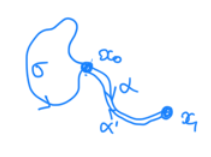
\includegraphics[scale=0.3]{images/conj_iso_grupos} 
\end{center}
\end{prop}
\begin{demo}
Fácil con las propiedades de \ref{sec:operaciones_con_caminos}.
\end{demo}

\section{Funtorialidad}%
\label{sec:funtorialidad}
\begin{defi}    
Definimos $h_*$ como:
\begin{align*}
    h: X \rightarrow Y &\text{ homeo, } h\left( x_0 \right) = y_0 \Rightarrow\\
    h_*: \pi\left( X, x_0 \right) &\rightarrow \pi\left( Y, y_0 \right) \text{ iso.}\\
    \left[ \sigma \right] &\mapsto \left[ h \circ \sigma \right] 
.\end{align*}
\end{defi}
Es fácil y útil: espacios homeomorfos deben tener grupos fundamentales isomorfos.

Por ejemplo, $\mathbb{S}^2$ y $\mathbb{R}P^2$ no son homeomorfos. Pero la construcción es mucho más general.
%TODO: Imagen
\begin{center}
    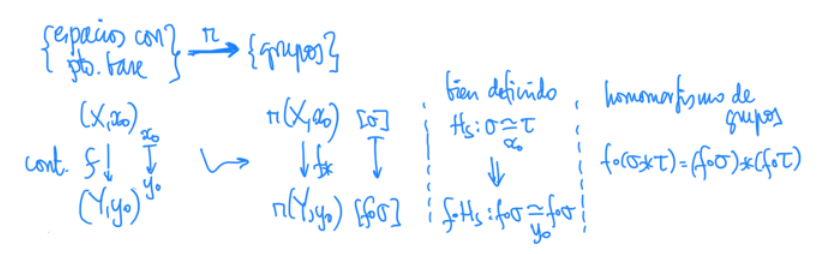
\includegraphics[scale=0.3]{images/const_functorialidad} 
\end{center}

\begin{defi}[Funtorialidad]
$\left( g \circ f \right)_* = g_* \circ f_*$ y $\left( id_X \right)_* = id_{\pi\left( X, x_0 \right)}$. 
\end{defi}

\begin{ej}
    Si $h: X \rightarrow Y,\ x_0 \mapsto y_0$ es homeomorfismo $\Rightarrow \left( h_* \right)^{-1} = \left( h^{-1} \right)_*$. [Más preciso que $h_*$ isomorfismo]
\end{ej}

\begin{prop}[Producto de espacios]
Tenemos que si:
%TODO: Imagen
\begin{center}
    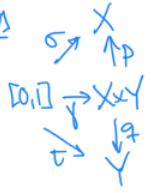
\includegraphics[scale=0.3]{images/prod_espacios_funt} 
\end{center} 
entonces:
\begin{align*}
    \pi\left( X \times Y, \left( x_0, y_0 \right) \right) &\xrightarrow{p_*, q_*} \pi\left( X, x_0 \right) \times \pi \left( Y, y_0 \right)\\
    \left[ \gamma \right] = \left[ \left( \sigma; \tau \right) \right] &\mapsto \left( \left[ \sigma \right], \left[ \tau \right] \right)
.\end{align*}
es un isomorfismo.
\end{prop}
\begin{demo}
Sean:
\[
\begin{rcases}
    F_s: \sigma_1 \stackrel{x_0}{\simeq} \sigma_2\\
    G_s: \tau_1 \stackrel{y_0}{\simeq} \tau_2
\end{rcases} \Rightarrow \left( F_s, G_s \right): \left( \sigma_1, \tau_1 \right) = \gamma_1 \mapsto \gamma_2 = \left( \sigma_2, \tau_2 \right) \text{ y nada más...} 
\]
\end{demo}

\begin{ej}
\begin{enumerate}
    \item $\pi\left( \mathbb{S} \times \mathbb{S} \right) = \pi\left( \mathbb{S} \right) \times \pi\left( \mathbb{S} \right) = \mathbb{Z}^2$.
    \item $\pi\left( \mathbb{S}^1 \times \left[ 0, 1 \right] \right) = \pi\left( \mathbb{S} \right) \times \pi\left( \left[ 0, 1 \right] \right)$.
\end{enumerate}
\end{ej}
